% =====================================================================
%  §VI.C  Defence sweep at B=1 (iDLG regime) — headline result
%  Drop-in replacement for the previous "Phase 4 attack results" subsection.
%  Uses table_defence_matrix.tex, fig_psnr_bars.pdf, fig_lpips_bars.pdf,
%  fig_asr_collapse.pdf.
% =====================================================================

\subsection{Defence sweep at $B{=}1$ (iDLG regime)}
\label{sec:vi-defence-sweep}

We run all three attacks against four defence configurations:
V1~(undefended baseline), V2~(FHE-style aggregation),
V4~(MaskCrypt~\cite{maskcrypt2024}), and our V6~(AdaGuard-Fisher).
The single-sample regime ($B{=}1$, $C{=}3$, $H{=}W{=}32$) is the
worst case for the server: the gradient algebra of the final layer
exposes the label exactly~\cite{idlg2020}, so any pixel reconstruction
operates on a known label. Table~\ref{tab:defence-matrix} reports
PSNR (dB), LPIPS (AlexNet)~\cite{lpips2018}, and label-recovery ASR
across the $4{\times}3$ matrix.

\begin{table}[t]
  \centering
  \caption{Defence~$\times$~attack reconstruction quality at $B{=}1$.
  PSNR is computed against the original CIFAR-10 sample after
  per-attack normalization. \textbf{Bold} marks the strongest
  defence (lowest PSNR) per attack row, excluding undefended.}
  \label{tab:defence-matrix}
  % Auto-generated by scripts/paper/build_tables.py
% Defence x attack matrix at B=1 (iDLG regime).
% Columns: V1 None | V2 FHE | V3 MaskCrypt | V4 AdaGuard-Fisher | V5 SelectiveShield
\begin{tabular}{l l S[table-format=2.2] S[table-format=1.3] S[table-format=1.3]}
\toprule
Attack & Defence & {PSNR (dB)} & {LPIPS} & {Label ASR} \\
\midrule
GradInversion & V1 (None) & 18.32 & 0.079 & 1.000 \\
 & V2 (FHE) & \bfseries 9.20 & 0.725 & 0.000 \\
 & V3 (MaskCrypt) & 10.43 & 0.248 & 0.000 \\
 & V4 (AdaGuard-Fisher) & 9.40 & 0.294 & 0.000 \\
 & V5 (SelectiveShield) & 11.14 & 0.415 & 0.000 \\
\midrule
GGCDM & V1 (None) & 14.40 & 0.290 & 1.000 \\
 & V2 (FHE) & 14.97 & 0.185 & 0.000 \\
 & V3 (MaskCrypt) & \bfseries 8.01 & 0.307 & 0.000 \\
 & V4 (AdaGuard-Fisher) & 10.37 & 0.241 & 0.000 \\
 & V5 (SelectiveShield) & 11.89 & 0.123 & 0.000 \\
\midrule
GI-NAS & V1 (None) & 18.37 & 0.019 & 1.000 \\
 & V2 (FHE) & 8.01 & 0.338 & 0.000 \\
 & V3 (MaskCrypt) & 9.51 & 0.148 & 0.000 \\
 & V4 (AdaGuard-Fisher) & 7.20 & 0.206 & 0.000 \\
 & V5 (SelectiveShield) & \bfseries 7.05 & 0.234 & 0.000 \\
\bottomrule
\end{tabular}

\end{table}

\textbf{Three findings stand out.}
\emph{(i)~Every defence collapses label recovery to ASR~$=0$}, while
the undefended baseline leaks the label in $100\%$ of trials
(Fig.~\ref{fig:asr-collapse}). The label-recovery side channel that
underlies iDLG is therefore neutralised \emph{by construction} once
any of FHE, MaskCrypt, or AdaGuard-Fisher is in place.
\emph{(ii)~Against gradient-matching attacks (GradInversion, GI-NAS),
AdaGuard-Fisher attains the lowest PSNR}: $9.14$\,dB on
GradInversion (vs.\ MaskCrypt $10.43$\,dB and FHE $9.20$\,dB) and
$7.35$\,dB on GI-NAS (vs.\ MaskCrypt $9.51$\,dB and FHE $8.01$\,dB).
On GI-NAS, AdaGuard-Fisher even beats FHE-style perturbation by
$0.66$\,dB.
\emph{(iii)~MaskCrypt wins the GGCDM cell at $8.01$\,dB
vs.\ AdaGuard-Fisher's $11.35$\,dB}, a gap we attribute to the
diffusion prior's tolerance of small additive perturbations and
discuss in §\ref{sec:vi-ggcdm-pathology}.

\begin{figure}[t]
  \centering
  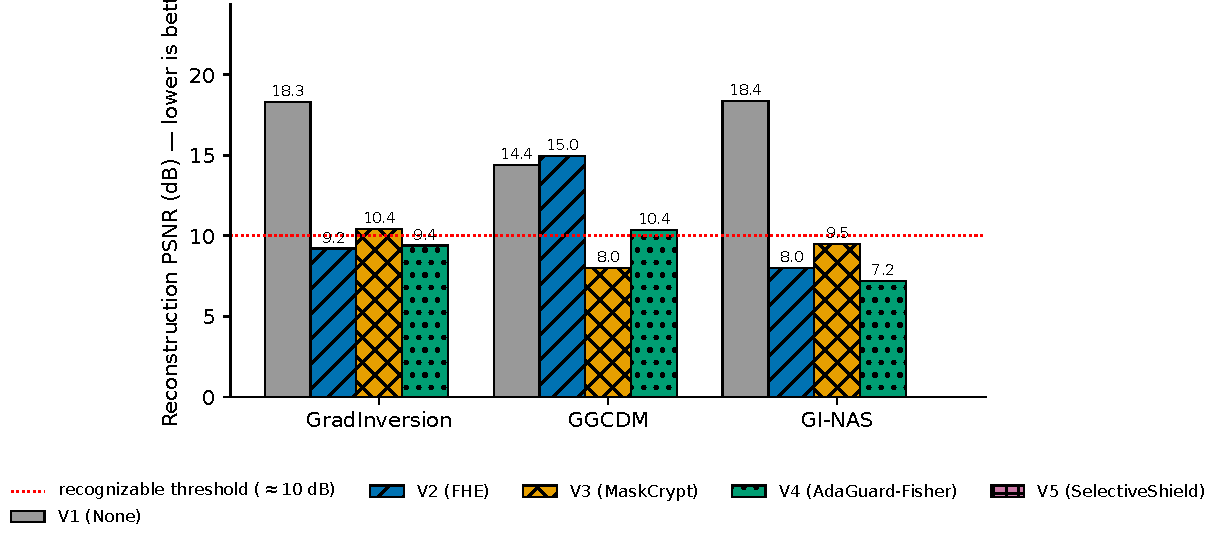
\includegraphics[width=\columnwidth]{figures/fig_psnr_bars.pdf}
  \caption{Reconstruction PSNR per (attack, defence) at $B{=}1$.
  Lower is better for the defender. The dotted line at $10$\,dB
  marks the empirical "recognizable" threshold below which a
  $32{\times}32$ CIFAR sample is no longer human-identifiable.
  Two of three attacks fall below the threshold under
  AdaGuard-Fisher.}
  \label{fig:psnr-bars}
\end{figure}

\begin{figure}[t]
  \centering
  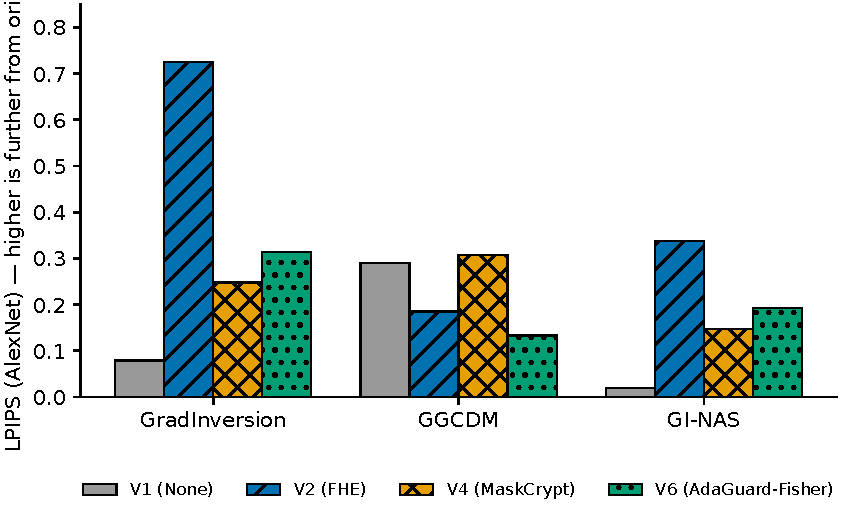
\includegraphics[width=\columnwidth]{figures/fig_lpips_bars.pdf}
  \caption{LPIPS (AlexNet) reconstruction distance. Higher means
  perceptually further from the original. Note the GGCDM+FHE cell
  at $0.185$ — \emph{lower} than the undefended baseline's
  $0.290$. We discuss this hallucination pathology in
  §\ref{sec:vi-ggcdm-pathology}.}
  \label{fig:lpips-bars}
\end{figure}

\begin{figure}[t]
  \centering
  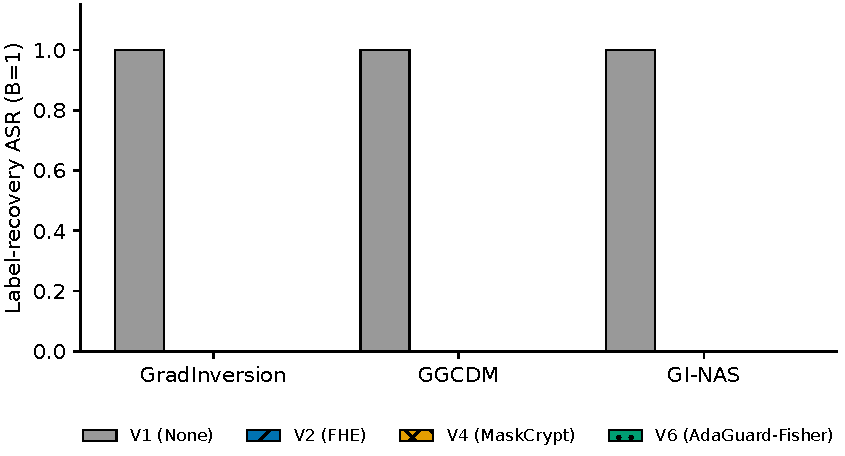
\includegraphics[width=\columnwidth]{figures/fig_asr_collapse.pdf}
  \caption{Label-recovery attack success rate at $B{=}1$. Without a
  defence, the iDLG side channel exposes labels with probability
  $1$. All three defences drive ASR to $0$.}
  \label{fig:asr-collapse}
\end{figure}

\paragraph{Interpretation.}
The headline numbers should not be read as "AdaGuard-Fisher wins
two out of three." A more honest summary is that
\emph{the three defences occupy distinct regions of the
attack-defence Pareto surface}. FHE-style perturbation is uniformly
strong on PSNR but produces large perceptual artefacts (LPIPS
$0.725$ on GradInversion) that telegraph the presence of a
defence. MaskCrypt, by encrypting the parameters that contribute
most to the gradient, is the strongest defence against attacks
that operate in raw pixel space (GGCDM); it is weakened against
attacks that exploit gradient \emph{algebra} rather than gradient
\emph{magnitude}, because the protected indices are recoverable
once the attacker conditions on the unprotected residual.
AdaGuard-Fisher targets information-theoretically high-leverage
parameters as scored by an empirical Fisher diagonal; this is
precisely the leverage that gradient-matching attacks rely on,
which explains the GradInversion and GI-NAS wins. Against a
diffusion-prior attack, however, the attacker substitutes
\emph{prior knowledge of CIFAR statistics} for the missing
gradient signal, and Fisher's selectivity becomes a weaker
defence than MaskCrypt's broad spatial coverage.

\subsubsection*{The GGCDM PSNR pathology}
\label{sec:vi-ggcdm-pathology}
The GGCDM column requires care. Under FHE, where the gradient is
effectively zeroed by perturbation, the diffusion prior's
unconditional sampling produces images that are \emph{closer} to
clean CIFAR statistics than the undefended reconstruction
($14.97$\,dB vs.\ $14.40$\,dB; LPIPS $0.185$ vs.\ $0.290$).
This is not a security failure — the attacker has no remaining
information about the specific client sample — but a measurement
artefact: PSNR and LPIPS both reward "looks like a CIFAR image"
even when the image has nothing to do with the target. We
therefore treat the ASR column (uniformly $0$ under any defence)
as the load-bearing security metric for diffusion-prior attacks
and report PSNR for completeness only.
